\NeedsTeXFormat{LaTeX2e}
\LoadClass{article}
\documentclass{article}

\usepackage{fancyhdr} % Required for custom headers
\usepackage{lastpage} % Required to determine the last page for the footer
\usepackage{extramarks} % Required for headers and footers
\usepackage[usenames,dvipsnames]{color} % Required for custom colors
\usepackage{graphicx} % Required to insert images
\usepackage{listings} % Required for insertion of code
\usepackage{courier} % Required for the courier font
\usepackage{booktabs}% http://ctan.org/pkg/booktabs
\usepackage{color, colortbl}
\usepackage{amsmath}
\usepackage{amssymb}
\usepackage{cancel}
\usepackage{breqn}

% Margins
\topmargin=-0.45in
\evensidemargin=0in
\oddsidemargin=0in
\textwidth=6.5in
\textheight=9.0in
\headsep=0.25in

\linespread{1.1} % Line spacing

\newcommand{\tabitem}{~~\llap{\textbullet}~~}
\newcommand{\tab}[1][0.5cm]{\hspace*{#1}}

\begin{document}
	
\section{Formulation: Part I}
Optimization equation
\begin{equation}\label{eq1}
	\text{min}\sum_{k\in N}\sum_{i\in I}\begin{pmatrix}\alpha \ln{Q_i(k)} + \boxed{\color{blue}c(k)P_{0i}(k)\color{black}} \end{pmatrix}
\end{equation}
$\alpha$ represents the cost associated with losing energy to capacity fade. Note that $Q_i$ represents the percent capacity fade for node \textit{i} at time step \textit{k}. $c(k)$ represents the cost to generate electricity. \\
We want to know \boxed{\textbf{whether implementing the boxed power cost term is appropriate}} . We want our problem to include a cost for drawing power from the grid in addition to losing charge capacity, but are unsure if this is ambitious. 
\begin{equation}\label{eq2}
	\ln{Q_i(k)} = \ln(B) - \frac{E_A}{RT_i(k)} + z\ln{\color{red}A_{h,i}(k)\color{black}} \quad \forall k\in 1..N, i\in 1..I
\end{equation}
Linearized version of the percent capacity loss expression. Note that $B, E_A, R, z$ are all constants based on battery kinetics. We note that $T_i$- the temperature of battery \textit{i}- could be a constant but here we present the temperature dynamics as well. The \color{red}red \color{black} term represents the amp-hour throughput, which is defined below:
\begin{equation}\label{eq3}
	A_{h,i} = \underset{\color{blue}k-indexed\color{black}}{\text{cycle number}}\cdot\underset{\frac{I_i\Delta t}{\color{blue}Q_{\text{max}}\color{black}}}{\text{DOD}}\cdot\underset{Q_{\text{max}}}{\text{full cell capacity}}
\end{equation}
Here are uncertain whether the \boxed{\textbf{cycle number and depth-of-discharge are accurately represented}}. Namely, the depth-of-discharge could be calculated relative to the current total capacity instead of the initial total capacity. If the expression is valid as written, then $A_{h,i}(k)$ is simply $I_i(k)\Delta t$. Now we describe the battery power dynamics:
\begin{equation}\label{eq4}
	E_i(k+1) = E_i(k) + p_{b,i}(k)\Delta t \quad \forall k\in 1..N, \forall i\in 1..I
\end{equation}
\begin{equation}\label{eq5}
	p_{b,i}(k) = P_{0i}(k) - d_i(k) \quad \forall k\in 1..N, \forall i\in 1..I
\end{equation}
\begin{equation}\label{eq6}
	\sum_{i\in I}P_{0i}(k) \leq G(k) \quad \forall k\in 1..N, \forall i\in 1..I
\end{equation}
Note quickly here that $p_{b,i}(k)$ is the battery power available at node \textit{i} at time step \textit{k}, $P_{0i}(k)$ is the power delivered to node \textit{i} at time step \textit{k}, and $d_i(k)$ is the demand at node \textit{i} at time step \textit{k}. $G(k)$ is the total power available from the grid at time step \textit{k}. Here we want to know whether\boxed{\textbf{power can be returned}} to the grid from the battery nodes.
\begin{equation}\label{eq7}
	E_{\text{min}} \leq E_i(k) \leq E_{\text{max}} \quad \forall k\in 1..N, i\in 1..I
\end{equation}

\section{Temperature dynamics}
\begin{equation}\label{eq8}
	\color{blue}C\color{black}\dot{T_i}(k) = \color{blue}h\color{black}\begin{pmatrix}T_i(k) - T_{\infty}\end{pmatrix} + R_BI_i(k)^2 \quad \forall k\in 1..N, i\in 1..I
\end{equation}
\begin{equation}\label{eq9}
	T_i(k)\dot{T_i}(k)\Delta t = T_i(k+1) \quad \forall k\in 1..N, i\in 1..I
\end{equation}
\begin{equation}\label{eq10}
	T_{\text{min}} \leq T_i(k) \leq T_{\text{max}} \quad \forall k\in 1..N, i\in 1..I
\end{equation}
Beyond the general question of whether we want to implement temperature dynamics or not, we wanted to know here the \boxed{\textbf{units of h and C}}.
\section{Formulation: Part II}
\begin{equation}\label{eq11}
	p_{b,i}(k) = I_i(k)\color{red}V_i(k)\color{black} \quad \forall k\in 1..N, i\in 1..I
\end{equation}
\begin{equation}\label{eq12}
	V_i(k) = \color{red}V_{oc,i}(k)\color{black} -I_i(k)R_B \quad \forall k\in 1..N, i\in 1..I
\end{equation}
\begin{equation}\label{eq13}
	V_{oc,i}(k) = \color{red}f(\text{SOC}_i(k))\color{black} \quad \forall k\in 1..N, i\in 1..I
\end{equation}
\begin{equation}\label{eq14}
	\text{SOC}_i(k) = \frac{E_i(k)}{\color{blue}Q_{\text{max}}\color{black}V_{oc,i}(k)}\quad \forall k\in 1..N, i\in 1..I
\end{equation}
Hopefully for these sets of equations the variables are self-illuminating. The main question here is from equation \color{red}\ref{eq14}\color{black} - \boxed{\textbf{is the \textit{Q} term $Q_{\text{max}}$ or $Q_{\text{cap, i}}$}}, as defined below?
\begin{equation}\label{eq15}
	Q_{\text{cap, i}}(k) = Q_{\text{max}}\begin{pmatrix}1-Q_i(k)\end{pmatrix} \quad \forall k\in 1..N, i\in 1..I
\end{equation}

\section{DP Formulation}
Let $V(k)$ represent the cumulative capacity fade and power generation from time step \textit{k} to total time \textit{N}. We define control variables $I_i(k)$ as $u_k \; \forall i$ and state variables $T_i(k)$ as $x_k \; \forall i$:
\begin{equation}\label{eq16}
	V_k(x_k) = \underset{u_k,x_k}{\text{min}}\begin{Bmatrix}\sum_{i\in I}\begin{pmatrix}\alpha \underset{\color{red}f(u_k, x_k)\color{black}}{\text{ln(Q(k))}} + c(k)P_{0i}(k)\end{pmatrix} + V(k+1) \end{Bmatrix}\quad \forall k\in 1..N
\end{equation}
We finally establish the boundary condition: \[V(N+1) = 0\] The only question here is whether \boxed{\textbf{$T_i$ or $\text{SOC}_i$}} represent the state variables.

\section{Detailed questions}
In summary, here are a detailed list of our questions:
\begin{itemize}
	\item Is implementing the power cost term appropriate? Will it complicate our solution to try to minimize the overall cost to draw power from the grid in addition to minimizing cumulative aging?
	\item What are the units of $\alpha$, h, and C?
	\item Is $Q_{\text{max}}$ or $Q_{\text{cap},i}$ in the denominator for the depth of discharge expression? What about for the state of charge?
	\item Is $P_{0i}$ strictly non-negative? (i.e. is power not returned to grid?)
	\item Will $T_i$ or $\text{SOC}_i$ be our state variable?
	\item Where can we get physical data for our constants and input data?
	\item What additional research can be done from literature? How can we boost that portion of our report?
	\item Is demand at each node \textit{i} only met by the node it is connected to? Are there other configurations we can explore? Please reference the picture below.
\end{itemize}
\begin{center}
	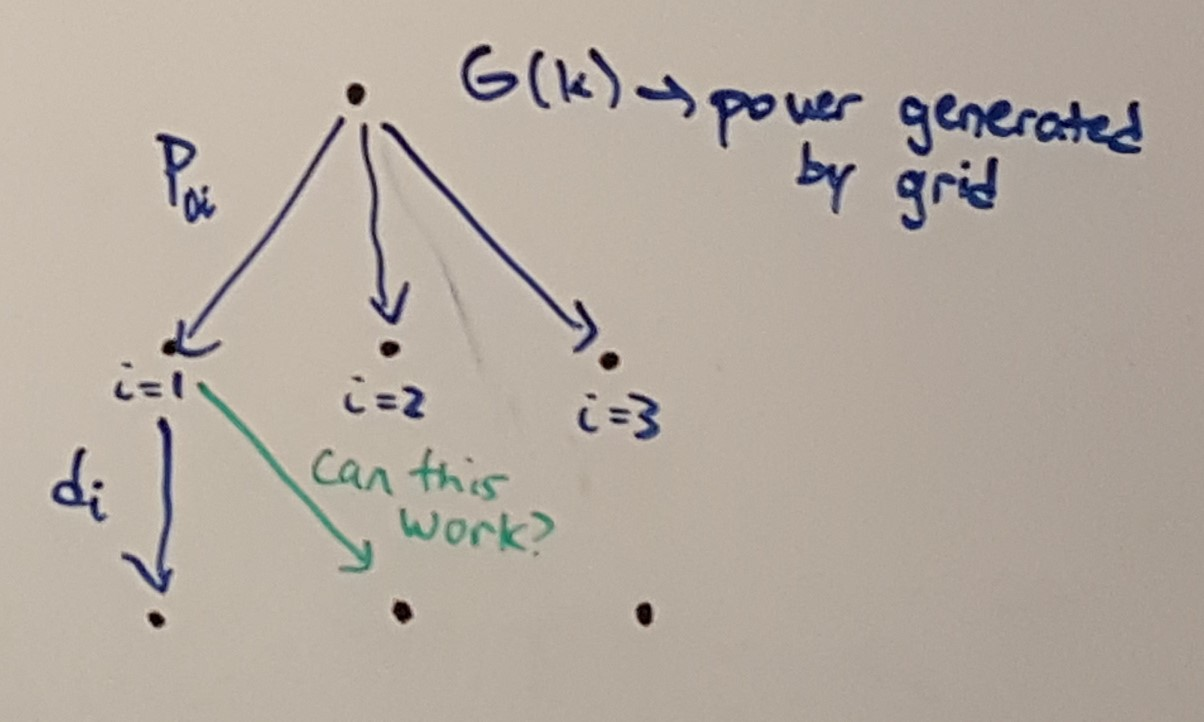
\includegraphics[width=0.7\textwidth]{grid.jpg}
\end{center}
We appreciate your time to read through this!
\end{document}